% This text is proprietary.
% It's a part of presentation made by myself.
% It may not used commercial.
% The noncommercial use such as private and study is free
% Sep. 2005 
% Author: Sascha Frank 
% University Freiburg 
% www.informatik.uni-freiburg.de/~frank/


\documentclass{beamer}
\usepackage{graphicx}
\usepackage{amsmath}
\usepackage{amssymb}
\usepackage{xcolor}
\definecolor{mygreen}{cmyk}{0.82,0.11,1,0.25}
\begin{document}
\title{Spring 2020 MAT303 Recitations}   
\author{Week of 4/13/20: Sections 3.5 and 3.6} 
\date{} 

\frame{\titlepage} 


\frame{\frametitle{Section 3.5: Nonhomogeneous Equations}

Our setup consists of a second-order differential equation with linear coefficients, \pause
\begin{equation*}
y''(t)+Py'(x)+Qy(x) = F(x),
\end{equation*}
\pause
where $P,Q$ are constants. \pause In today's lecture we will learn how to solve this via Variation of Parameters, by perturbing its complementary solutions.
}

\frame{\frametitle{Section 3.5: Nonhomogeneous Equations}

Assume that a complementary solution to our equation takes the form
\begin{equation*}
y_c(x)=C_1y_1(x)+C_2y_2(x),
\end{equation*}
\pause
where $y_1$ and $y_2$ are linearly independent, $C_1,C_2$ are constants. 
\pause 
\vspace{0.1in}

The method of variation of parameters consists of a perturbation of the complementary solution of the type
\begin{equation*}
y(x)=u_1(x)y_1(x)+u_2(x)y_2(x),
\end{equation*}
\pause
where $u_1, u_2$ are \emph{functions} of $x$ to be determined.
}

\frame{\frametitle{Section 3.5: Nonhomogeneous Equations}
Consider the equation
\begin{equation*}
y^{''} + y = e^x.
\end{equation*}
\pause 
\vspace{0.1in}
The characteristic polynomial of its homogeneous counterpart is $p(r)=r^2+1$, with complex roots $\pm i$. \pause The complementary solution of the problem is 
\begin{equation*}
y_c(x)=A_1\cos(x)+A_2\sin(x).
\end{equation*}\pause
We perturb it by setting 
\begin{equation*}
y(x)=u_1(x)\cos(x)+u_2(x)\sin(x),
\end{equation*}
\pause
for unknown functions $u_1,u_2$. 
}

\frame{\frametitle{Section 3.5: Nonhomogeneous Equations}
Finding the functions $u_1$ and $u_2$ amounts to using a system of lower-order equations.\pause The derivative of this guess is 
\begin{equation*}
y^{'}(x)=[u_{1}^{'}(x)\cos(x)+u_{2}^{'}(x)\sin(x)] -u_1(x)\sin(x)+u_2(x)\cos(x).
\end{equation*}
\pause 
which involves derivatives of $u_1$ and $u_2$. \pause We impose a condition that removes them from the equation:
\begin{equation*}
u_{1}^{'}(x)\cos(x)+u_{2}^{'}\sin(x)=0.
\end{equation*}
\pause 
This is the first equation of our system.
}

\frame{\frametitle{Section 3.5: Nonhomogeneous Equations}
We will continue our derivation of  $y$ and its derivatives under this assumption, that is, \pause
\begin{equation*}
y^{'}(x)= -u_1(x)\sin(x)+u_2(x)\cos(x),
\end{equation*}
\pause
so that 
\begin{equation*}
y^{''}(x) = -u_{x}^{'}(x)\sin(x)-u_1(x)\cos(x)+u_{2}^{'}(x)\cos(x)-u_2(x)\sin(x).
\end{equation*}
\pause
It follows that 
\begin{align*}
y^{''}(x)+y(x) & =-u_{1}^{'}(x)\sin(x)+u_{2}^{'}(x)\cos(x) \\
e^{x} & = -u_{1}^{'}(x)\sin(x)+u_{2}^{'}(x)\cos(x) .
\end{align*}
}

\frame{\frametitle{Section 3.5: Nonhomogeneous Equations}
The desited system of linear, first-order equations on $u_1,u_2$ is
\begin{align*}
u_{1}^{'}(x)\cos(x)+u_{2}^{'}(x)\sin(x) & =0\\
-u_{1}^{'}(x)\sin(x)+u_{2}^{'}(x)\cos(x) & = e^{x}.
\end{align*}
\pause
We note that the determinant of this system is the Wronskian of the complementary solutions, $\cos(x), \sin(x)$, \pause and their linear independence tell us the system is solvable by elimination.  
\pause 
The solutions are
\begin{align*}
u_1(x) & = \frac{e^{x}(\cos(x)-\sin(x))}{2} + A_1, \\
u_2(x) & = \frac{e^{x}(\sin(x)+\cos(x))}{2}+ A_2.
\end{align*}
}

\frame{\frametitle{Section 3.5: Nonhomogeneous Equations}
The final step is to combine the auxilliary functions $u_1$, $u_2$ and the complementary solutions, to obtain
\begin{align*}
y(x) & = u_1(x)\cos(x)+u_2(x)\sin(x) \\
& = \frac{e^x}{2}+A\cos(x)+B\sin(x)
\end{align*}

Try to confirm this answer by Undetermined Coefficients!
}

\frame{\frametitle{Section 3.5: Nonhomogeneous Equations}
In problem 3.5.54, we have a case in which Undetermined Coefficients doesn't work, the equation
\begin{equation*}
y^{''}(x)+y(x) = \csc^2(x).
\end{equation*}
\pause
As in example 1, the complementary solution is 
\begin{equation*}
y_c(x)=A_1\cos(x)+A_2\sin(x),
\end{equation*}
\pause
so we perturb it by setting 
\begin{equation*}
y(x)=u_1(x)\cos(x)+u_2(x)\sin(x).
\end{equation*}
}

\frame{\frametitle{Section 3.5: Nonhomogeneous Equations}
Here the functions $u_1$, $u_2$ have to satify the system
\begin{align*}
u_{1}^{'}(x)\cos(x)+u_{2}^{'}(x)\sin(x) & =0\\
-u_{1}^{'}(x)\sin(x)+u_{2}^{'}(x)\cos(x) & = \csc^2(x).
\end{align*}
\pause
By elimination we find 
\begin{align*}
u_{1}^{'}(x) & = \log(\cot(x)+\csc(x))+A_1,\\
u_{2}^{'}(x) & = -\csc(x)+A_2.
\end{align*}
\pause
So the final solution is 
\begin{equation*}
y(x)=A_1\cos(x) + A_2\sin(x) + \log(\cot(x)+\csc(x))\cos(x)-1.
\end{equation*}
}

\frame{\frametitle{Section 3.6: Forced Oscillations}
In problem 3.6.2, we are given a differential equation
\begin{equation*}
x^{''}+4x=5\sin(3t),
\end{equation*}
with initial conditions $x(0)=0,x^{'}(0)=0$.
\pause
\vspace{0.1in}
The general complementary solution to the problem takes the form
\begin{equation*}
x_c(t)=A\cos(2t)+B\sin(2t),
\end{equation*}
\pause
whereas one expects a particular solutions to be written as 
\begin{equation*}
x_p(t)=C_1\sin(3t)+C_2\cos(3t).
\end{equation*}
}

\frame{\frametitle{Section 3.6: Forced Oscillations}
In problem 3.6.2, we are given a differential equation
\begin{equation*}
x^{''}+4x=5\sin(3t),
\end{equation*}
with initial conditions $x(0)=0,x^{'}(0)=0$.
\pause
\vspace{0.1in}
The general complementary solution to the problem takes the form
\begin{equation*}
x_c(t)=A\cos(2t)+B\sin(2t),
\end{equation*}
\pause
whereas one expects a particular solutions to be written as 
\begin{equation*}
x_p(t)=C_1\sin(3t)+C_2\cos(3t).
\end{equation*}
}

\frame{\frametitle{Section 3.6: Forced Oscillations}
Using the method of Undetermined Coefficients, we find the values $C_1=-1$ and $C_2=0$, thus the inhomogeneous solution is
\begin{equation*}
x(t)=A\cos(2t)+B\sin(2t) -\sin(3t).
\end{equation*}
\pause
The coefficients $A$ and $B$ are found by matching the initial data.\pause We observe that 
\begin{equation*}
x^{'}(t)=-2A\sin(2t)+2B\cos(2t)-3\cos(3t),
\end{equation*}
\pause
so that the conditions at $t=0$ amount to 
\begin{align*}
 A  & = 0 \\ 
 2B-3 & = 0,
\end{align*}
\pause
which gives
\begin{equation*}
x(t)=\frac{3}{2}\sin(2t)-\sin(3t),
\end{equation*}
a periodic function with period $2\pi$.
}

\frame{\frametitle{Section 3.6: Forced Oscillations}
 Below is a plot of its graph, the marked points corresponding to periods.
\begin{center}
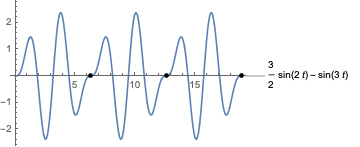
\includegraphics[width=0.8\textwidth]{p3.png} 
\end{center}
}
%
%\section{Section no.3} 
%\subsection{Tables}
%\frame{\frametitle{Tables}
%\begin{tabular}{|c|c|c|}
%\hline
%\textbf{Date} & \textbf{Instructor} & \textbf{Title} \\
%\hline
%WS 04/05 & Sascha Frank & First steps with  \LaTeX  \\
%\hline
%SS 05 & Sascha Frank & \LaTeX \ Course serial \\
%\hline
%\end{tabular}}
%
%
%\frame{\frametitle{Tables with pause}
%\begin{tabular}{c c c}
%A & B & C \\ 
%\pause 
%1 & 2 & 3 \\  
%\pause 
%A & B & C \\ 
%\end{tabular} }
%
%
%\section{Section no. 4}
%\subsection{blocs}
%\frame{\frametitle{blocs}
%
%\begin{block}{title of the bloc}
%bloc text
%\end{block}
%
%\begin{exampleblock}{title of the bloc}
%bloc text
%\end{exampleblock}
%
%
%\begin{alertblock}{title of the bloc}
%bloc text
%\end{alertblock}
%}
\end{document}


